\chapter{Wortschatz2DBpedia}\label{sec:wortschatz2dbpedia}

\begin{dfn}
\emph{"`Ein \emph{Mapping}\footnote{engl. mapping [comp.] = Abbildung,Zuordnung} ist eine Menge paarweiser Zuordnungen, sogenannter Korrespondenzen, zwischen Instanzdaten.
Dabei wird in dieser Arbeit mit dem Begriff Korrespondenz nicht nur die Verknüpfung gleicher Objekte gemeint, sondern allgemein eine Beziehung zwischen zwei Objekten ausgedrückt."'}\citep{thor-dissertation}

%Diese Definition ist der Dissertation von Dr. Andreas Thor entnommen .
Ein Mapping erlaubt damit komplexe Anfragen, die mit den Datenquellen allein nicht möglich wären.
Es erlaubt auch die Aggregation von Informationen verschiedener Art über ein Objekt.\footnote{in dieser Arbeit sowohl statistische als auch semantische Informationen über Wörter}
\end{dfn}

\section{Anforderungen}\label{sec:anforderungen}
%1239916 wortschatz2dbpedia/input/wortschatz/en_words_all.txt

Aufgabe ist es, ein Programm zu implementieren, welches ein Mapping zwischen dem \emph{Projekt Deutscher Wortschatz} (sowie seiner internationalen Version) und der \emph{DBpedia} generiert.
Eine solche Verknüpfung verbindet jeweils eine Ressource des Wortschatzes mit einer Ressource der DBpedia.
Eine Ressource beim Wortschatz ist eine Wortform. Eine DBpedia-Ressource ist eine RDF-Entität, welche automatisch extrahierte strukturierte Informationen aus einem Wikipediaartikel enthält und 
dabei ein Objekt oder Konzept aus der realen Welt beschreibt.
Das Programm muss einmal pro Jahr von einer Fachkraft ausgeführt werden, um mit den jährlich aktualisierten Wortschatzdaten ein neues Mapping herzustellen.
Die Anforderungsanalyse ergab dabei Folgendes:

\subsection{Funktionale Anforderungen}
Aufgabe des Programmes ist die Erstellung eines Mappings zwischen DBpedia und dem Internationalen Wortschatzprojekt in einer bestimmten Sprache.
Das Mapping besteht aus Links zwischen Wörtern des Wortschatzprojektes und Ressourcen der DBpedia.
Dabei sind zunächst einmal nur die englischen und deutschen Versionen zu verarbeiten, eine einfache Erweiterung auf andere Sprachen soll jedoch garantiert sein.
Die Wörter entstammen dem Corpus des Wortschatzprojektes und enthalten daher sowohl Einzelne- ("`\emph{Brot}"'), als auch Mehrwörter ("`\emph{SPD Generalvorsitzender Frank Walter Steinmeyer}"'),
 wie sie im normalen schriftlichen Gebrauch ausgewählter Quellen (Zeitungen und zufällig ausgewählte Webseiten) enthalten sind.
Die DBpedia-Ressource eines bestimmten Namens ist eine RDF-Entität, welche automatisch extrahierte, strukturierte maschinenverarbeitbare Informationen 
aus dem gleichnamigen Wikipediaartikel enthält und damit ein Objekt oder allgemeiner ein Konzept der realen Welt repräsentiert.
\begin{center}
\begin{tabular}{ll}
\toprule
DBpedia-Ressource & \url{dbpedia:London_Heathrow_Airport}\\
rdfs:label & London Heathrow Airport\\
Wikipedia Titel & London Heathrow Airport\\
Wikipedia URL & \url{en-wiki:London_Heathrow_Airport}\\
\bottomrule
\end{tabular}
\end{center}

\begin{dfn}\label{dfn:korrekte_korrespondenz}
Ein Paar $(w,a)$, wobei $w$ eine Wortform des englischen Wortschatzes und $a$ ein Artikelname der englischen Wikipedia ist, ist eine \emph{Korrespondenz}.
Es existiert dann sowohl ein Wikipediaartikel \article{en-wiki:}$a$ als auch eine DBpedia-Entität \article{dbpedia:}$a$.
Eine Korrespondenz gilt genau dann als \emph{korrekt}, wenn das Konzept, das von der Entität beschrieben wird, mit der Wortform benannt werden kann.
Das Konzept ist dann eine der möglichen Bedeutungen des Wortes.
\end{dfn}

Ist der Titel eines Wikipediaartikels mit einer Wortform identisch, dann bilden der Artikelname und die Wortform einen korrekten Link, da ein Titel eine Form der Benennung ist.
Da ein Titel aber immer groß geschrieben wird, sind hier zwei Arten von Fehlern möglich:
\begin{enumerate}
 \item Die Wortform ist identisch mit dem Artikelname, dieser wird jedoch normalerweise klein geschrieben, das Paar ist also inkorrekt.
 \item Die Wortform wird klein geschrieben, ist aber ansonsten identisch mit dem normalerweise klein geschriebenen Artikelnamen, das korrekte Paar wird also nicht erkannt.
\end{enumerate}
Da es jedoch keine Möglichkeit gibt, die wirkliche Großschreibung des ersten Buchstabens des Titels herauszufinden, wird die Großschreibung des ersten Buchstabens ignoriert und auch Paare mit 
verschiedener Großschreibung des ersten Buchstabens werden als identisch betrachtet.
Trotzdem wird in der Analyse in Abschnitt \ref{sec:analyse} die Präzision groß- und kleingeschriebener Wortformen getrennt aufgeschlüsselt, wobei das Existieren des Artikelnamens als Benennung ignoriert wird
(sonst hätten ja alle diese Paare nach Definition \ref{dfn:korrekte_korrespondenz} eine Präzision von \valunit{100}{\%}).

Ein solches minimales Mapping, das genau die identischen Paare umfasst ist leicht erzeugbar, %(\valunit{100}{\%} nach Definition \ref{dfn:korrekte_korrespondenz}),
enhält aber nur wenige Korrespondenzen (\val{13798} mit den Eingabedaten, die in Abschnitt \ref{sec:analyse} verwendet werden, also \valunit{11.6437}{\%} des dort erzeugten groben Mappings).
Durch verschiedene Methoden können auch nicht identische Paare mit gleicher Bedeutung gefunden werden.
Eine Möglichkeit dies zu tun ist, eine Ähnlichkeitsfunktion \s{} einzuführen, welche für eine Korrespondenz $(w,a)$ eine reelle Zahl zwischen $0$ (komplett verschieden) und $1$ (exakt gleich) annimmt.
Für jedes Wort $w$ und jeden Artikelnamen $a$ solch eine Ähnlichkeitsfunktion $\s(w,a)$ auszuwerten, würde jedoch zu einer aufgrund der großen Datenmenge nicht akzeptablen quadratischen Laufzeit führen,
denn bei einer groben Schätzung mit drei Millionen Wörtern\footnote{In der Analyse wurde nur das englische Normkorpus mit einer Million Sätzen verwendet, das gesamte Korpus ist jedoch wesentlich größer.}
und DBpedia-Ressourcen sowie angenommenen einer Million Vergleichen pro Sekunde ergibt sich eine Laufzeit von $3\frac{1}{2}$
Monaten.\footnote{$\frac{(3\cdot 10^6)^2\textnormal{Vergleiche}}{10^6 \textnormal{Vergleiche/s}} = 9 \cdot 10^6 \textnormal{s}$}


%\subsubsection{Stringtransformatoren}
Aus Laufzeitgründen soll das erweiterte Matching über die Entfernung von für die Wortdifferenzierung unwichtigen Merkmalen erfolgen.
Dies geschieht, in dem vor dem Matching eine Funktion $t: \textnormal{String} \rightarrow \pow{\textnormal{String}}$ (hier als \emph{Stringtransformator} bezeichnet) auf $w$ und $a$ ausgeführt wird.
Nun werden dem Matching alle Paare $(x,y), x \in \func{t}(w), y \in \func{t}(a)$, hinzugefügt. Dieser Vorgang wird auch als \emph{Termnormalisierung} bezeichnet.
Da die meisten in dieser Arbeit benutzten Stringtransformatoren immer einelementige Ergebnismengen erzeugen, werden diese aus Übersichtsgründen im Folgenden auch 
als Funktionen vom Typ $\textnormal{String} \rightarrow \textnormal{String}$ und einelementige Mengen als einzelne Zeichenketten dargestellt .
%Welche dieser Stringtransformatoren das beste Ergebnis bringen, wird mithilfe einer manuellen Analyse in Abschnitt \ref{sec:analyse} bestimmt.

\begin{bsp}
Sei $\func{t}=\func{String.toLowerCase()}$. Beim Matching wird nun die Groß- und Kleinschreibung ignoriert und das Paar (Cattle,cattle) gefunden.
\end{bsp}

Es sind auch Transformatoren möglich, die bestimmte Wortmengen ausschließen, deren Präzision sich als niedrig herausstellt,
indem sie diese Wörter auf das leere Wort $\epsilon$ abbilden, welches von der weiteren Verarbeitung ausgenommen ist.
Diese Transformatorfunktionen sollen auch vom Benutzer frei ausgewählt werden, auch die Hintereinanderausführung $\func{t}_1(\func{t}_2(...\func{t}_n(w)...)$ sowie das Vereinigen von Matches mit verschieden Transformatoren soll möglich sein. 
Welche dieser Methoden letztendlich verwendet werden, ergibt sich aus deren Analyse in Abschnitt \ref{sec:analyse}.

\iffalse
Eine Anwendung wäre das Einblenden der zu einem Wort zugeordneten Ressourcen mit Hilfe eines Links auf der Wortschatzseite zu diesem Wort, sodass sich ein Nutzer des Wortschatzes über die Bedeutung eines Wortes informieren kann.
Laut Herrn Volker Böhlke\footnotetext{http://www.informatik.uni-leipzig.de/personal/VBoehlke.html}, einem Mitarbeiter des Wortschatzprojektes, sind es die Nutzer einschlägiger Suchmaschinen gewöhnt, dass sie mehrere Möglichkeiten haben  um dann selbst den für sie geeignetsten Treffer auszuwählen.
In diesem Fall ist es daher besser, einen Anteil unpassender Verweise dabei zu haben, als das Risiko einzugehen, dass das Gesuchte nicht dabei ist.
Beim Einsatz in einer Kette von Verarbeitungsschritten, wie in Abschnitt \ref{sec:disambiguierung} beschrieben im Rahmen einer Wortsinndisambiguierung, können falsche Matches jedoch unerwünschte Fehlausgaben des Programmes liefern.
Aus diesen Gründen soll es zwei Typen von Links geben: diejenigen, bei denen eine hohe - (der sichere Link) und jene, bei denen eine etwas niedrigere Präzision erwartet wird (der alternative Link).
Als Grundlage kann von einem sicheren Link $(r,w)$ ausgegangen werden, wenn das Wort $w$ mit dem Namen $r$ der DBpedia-Ressource übereinstimmt, $r=w$. Dies sollte sich in linearer - und damit akzeptabler - 
Laufzeit implementieren lassen\footnote{Pseudocode: \code{für alle e aus Menge1: if(Menge2 enthält e) Mapping.add(e,e)}. Wenn Menge2 in einer Hash-basierten Datenstruktur gehalten wird, ist ein Zugriff in konstanter Zeit möglich.}.
Der Namen der Ressource ist ja auch der Name eines Artikels über das beschriebene Konzept, und damit ist $r$ und damit auch $w$ eine Benennung des Konzeptes.
Um die Coverage zu erhöhen, ist nun der nächste Schritt das Verknüpfen von Wörtern mit DBpedia-Ressourcen, deren Name nur noch ähnlich aber nichtmehr exakt gleich ist.
\fi

\subsubsection{Korrektheit}
Das Programm soll die ausgewählten Matchingroutinen natürlich fehlerfrei ausführen.
Aufgrund der großen Menge an Eingabedaten in der Größenordnung von mehreren Millionen und der Komplexität des Problems ist jedoch eine gewisse Menge an Fehlverknüpfungen unvermeidlich.
%Außerdem ist es schon eine Herausforderung an sich, eine exakte Definition zu finden, wann eine Verknüpfung korrekt ist [siehe insert verweis here], und diese anhand einer großen Zahl von Verknüpfungen zur  Überprüfung anzuwenden.
Bestimmte Verfahren besitzen zwar eine gewisse Fehlerquote, können jedoch den Anteil der gefundenen Verknüpfungen, die Coverage, wesentlich erhöhen.
Andere Methoden können zwar einige wenige weitere Verknüpfungen finden oder Fehlerhafte vermeiden, würden jedoch die Performance oder Entwicklungszeit unverhältnismäßig erhöhen.
Es muss also ein Kompromiss zwischen Laufzeit, Präzision, Coverage und Entwicklungszeit gefunden werden.
Links mit erwarteter hoher bzw. niedrigerer Präzision sind jedoch durch verschiedene Linktypen zu kennzeichnen.
%Auch wenn wir kaum Anforderungen an Geschwindigkeit stellen, würde aufgrund der großen Datenmenge ein Algorithmus quadratischer Laufzeitkomplexität (wie er vorliegt, wenn wir jedes Element der Einen mit jedem Element 
%der anderen Menge vergleichen) eine nicht tolerierbare Ausführungszeit haben.

\subsubsection{Redirects}
Das Matching soll auch Wikipedia - Redirects mit einbeziehen.
Redirects sind keine richtigen Artikel sondern nur Weiterleitungen.
Wenn man beim englischen Wikipedia \zb{} "`cow"' eingibt, wird man auf den Artikel "`cattle"' weitergeleitet.
Dies wird auch bei der Extraktion des Artikels zur DBpedia-Ressource vermerkt.
Diese Redirects sollen dabei für den Matchingvorgang wie normale Ressourcen betrachtet werden, danach aber auf das Ziel des Redirects geändert werden.

\begin{bsp}
Die Wortform "`cow"' wird untersucht, eine passende Ressource wird nicht gefunden, jedoch existiert der redirect \emph{cow}$\rightarrow$\emph{cattle},
\emph{cow} wird also erst auf \emph{cow} gemappt, hinterher jedoch werden die Redirects aufgelöst und das Paar wird zu $(\emph{cow},\emph{cattle})$ geändert.
\end{bsp}

\subsubsection{Mehrwortbegriffe}
Mehrwortbegriffe werden auch mit einbezogen, ein mögliches Mapping wäre (Franz Müntefering,Franz Müntefering).
Das Matching von Mehrwortbegriffen, die in anderen enthalten sind, soll nicht vorgenommen werden.
Mappings wie ((der) SPD Vorsitzende Franz Müntefering,Franz Müntefering) sind zwar richtig, müssen aber aufgrund des nicht angemessenen technischen Aufwandes nicht berücksichtigt werden.
Nehmen wir an, wir vergleichen den Mehrwortbegriff "`Gartenvorstand Peter Müller"' und eine Ressource namens "`Peter Müller"'.
Ob dieses Paar in unserem Sinne korrekt ist hängt nun davon ab, ob der Artikel tatsächlich einen Peter Müller beschreibt, der auch Gartenvorstand ist.
Dies lässt sich alleine aus dem Artikelnamen ohne Zusatzwissen jedoch nicht herausfinden.
Eine Möglichkeit wäre zwar, den Artikel nach dem Mehrwort "`Gartenvorstand Peter Müller"' zu durchsuchen, aber dann würde man immer noch Sätze wie 
"`es handelt sich in diesem Artikel nicht um den Gartenvorstand Peter Müller"' erkennen.
Das Vorkommen derartiger Matches wird dem Aufwand nicht entsprechend geschätzt, trotzdem soll die Möglichkeit, das Programm später auf Derartiges zu erweitern gegeben sein.

\subsection{Nichtfunktionale Anforderungen}

\subsubsection{Zuverlässigkeit}
Es werden keine Anforderungen an die Fehlertoleranz gegenüber Benutzereingabefehlern gestellt.
Eine Fehlermeldung ("`Ihre Eingabedatei besitzt ein ungültiges Format"') genügt.
Einzelne Fehleinträge in den Eingabedaten sollen jedoch nicht zum Abbruch des Programmes führen, sondern einfach ignoriert werden.

\subsubsection{Aussehen und Handhabung}
Es werden keine Anforderungen an das Aussehen und die Handhabung gestellt.
Eine Bedienung per Kommandozeile mit einer Ausgabe der zu erwarteten Parameter bei Fehleingabe genügt.

\subsubsection{Benutzbarkeit}
Es werden keine Anforderungen an das Aussehen und die Handhabung gestellt.

\subsubsection{Leistung und Effizienz}
Es werden keine signifikanten Anforderungen an die Laufzeit des Programmes gestellt, Laufzeiten von bis zu mehreren Tagen sind also explizit erlaubt. In solch einem Fall muss aber eine Vorschau implementiert werden.

\subsubsection{Betrieb und Umgebungsbedingungen}
Das Programm ist in Java zu implementieren und sollte daher überall laufen, wo eine standardkonforme Java Virtual Machine vorhanden ist.
Betrieben wird das Programm jedoch am Ende wohl auf einer Windows- oder Linuxplattform, sodass nur diese beiden zu garantieren und zu testen sind.

\subsubsection{Wartbarkeit, Änderbarkeit}
%Laut Herrn Boehlke wird im Wortschatzprojekt immer noch ein Programm eingesetzt, welches im Rahmen einer Diplomarbeit von vor über 10 Jahren entstand
%Dieses wird heute noch genutzt, aufgrund fehlender Analysierbarkeit und Erweiterbarkeit ist es jedoch mittlerweile Anfang einer Kette von Scripts, welche dessen Ausgabe im ursprünglich erforderlichen Format aufbereiten und in das mittlerweile Erforderliche bringen.
%Auch wenn der Autor nicht weiss, ob sein Programm ähnlich lange in Gebrauch sein wird, hofft er doch, dass ihm ein ähnliches Schicksal erspart bleibt.
Das Wortschatzprojekt besteht bereits seit über 10 Jahren und wird aufgrund seiner Popularität wohl noch lange in Gebrauch sein.
Die DBpedia nimmt eine zentrale Rolle für Linked Data ein.
Aus diesem Grunde soll das Programm auf erwartete Änderungen vorbereitet sein.
Eine ordentliche Umsetzung objektorientierter Prinzipien und Design Patterns wird also vorausgesetzt.
Insbesondere die Datenquellen und Vergleichsalgorithmen sollen ohne weitere Kenntnisse der Programmstruktur trivial erweiterbar sein.
Bestehende Programmroutinen müssen jedoch nur ein Grundmaß an Kommentaren aufweisen, welches erwartete Eingabe, Funktion und Ausgabe jedes Moduls beschreibt.
Es werden keine signifikanten Anforderungen an die Analysierbarkeit des Programmes gestellt.

\subsubsection{Portierbarkeit und Übertragbarkeit}
Es werden keine Anforderungen an die Portierbarkeit gestellt, aufgrund der Implementierung in Java ist diese jedoch ohne weiteren Aufwand gegeben.
Es reicht eine einfache Readme-Datei, welche den Installationsvorgang erklärt.
Die Sprache sowohl des Quelltextes, der Benutzerschnittstelle als auch der Dokumentation kann zwischen deutsch und englisch frei gewählt werden.

\subsubsection{Sicherheitsanforderungen}
Da Teile des Wortschatzes nicht frei verfügbar sind, dürfen diese Teile nicht in frei zugänglichen Distributionen des Programmes enthalten sein.
Weiterhin dürfen die geschützten Daten auch nicht aus dem Programm generierbar sein, falls es auf diese keinen Zugriff hat.
%Dieser Fall ist daher möglich, da bestimmte Informationen im Einzelzugriff frei verfügbar, in einer Komplettfassung jedoch kostenpflichtig sind.

\subsubsection{Flexibilität}
Das Programm soll die Daten so akzeptieren, wie sie auf der Webseite der DBpedia\footnote{\url{http://wiki.dbpedia.org/Downloads}} und des Wortschatzes\footnote{\url{http://corpora.informatik.uni-leipzig.de/download.html}} herunterladbar sind.
Falls sich deren Format ändert, soll es auf einfache Art und Weise so erweiterbar sein, dass es dieses verarbeiten kann.
Die Programmparameter sind aus einer Datei im INI-Format auszulesen.

\subsubsection{Skalierbarkeit}
Das Programm soll in der Lage sein, mit Datenmengen von mehreren Millionen Wörtern und DBpedia-Ressourcen umzugehen.

%\subsubsection{Entwicklungsdauer}
%Die Entwicklungsdauer sollte einen Monat nicht wesentlich überschreiten.
\section{Analyse}\label{sec:analyse}
Im Folgenden wird ein Mapping des Prototypen mit \val{118425} Einträgen analysiert, bei dessen Erstellung die \val{260880} Wörter des englischen Normcorpus mit einer Million Sätzen und \val{3201391} Artikelnamen miteinander verglichen wurden.

\subsection{Das Matching}
Der Matching läuft immer auf die gleiche Art und Weise ab:
Es werden die Datenquellen für den Wortschatz $D_w$ und die DBpedia $D_d$ festgelegt und ein Stringtransformator t ausgewählt.
Danach wird der Stringtransformator auf die Wortlisten der beiden Datenquellen angewendet und alle Paare $(a,w)$, $a\in D_d$, $w\in D_w$ mit $\func{t}(a)=\func{t}(w)$ werden dem Mapping hinzugefügt.
Üblicherweise ist dieser Stringtransformator eine Instanz der Klasse StringTransformatorList, das heißt eine Hintereinanderausführung mehrerer Stringtransformatoren.
Für die Stichprobenanalyse wird ein sehr grobes Mapping verwendet, das möglichst viele Paare abdeckt. Eine Auswertung der Präzision dieses Mappings und seiner Teile bestimmt, welche Stringtransformatoren für das
Erstellen des finalen Mappings letztendlich verwendet werden.
%Da eine Stichprobenanalyse sehr zeitaufwändig ist, wurde ein sehr grobes Mapping erzeugt, welches möglichst alle folgenden Mappings enthalten sollte, auch wenn dies zu Lasten der Präzision geht.
\paragraph{}
Die Eingabedaten sind:
\begin{itemize}
\item die zu diesem Zeitpunkt\footnote{Datum des Dumps: 20.5.2009} komplette Artikelliste der englischen DBpedia\footnote{\url{http://downloads.dbpedia.org/3.3/en/articles_label_en.csv.bz2}}
\item die Wörter aus einem Teilcorpus\footnote{\url{http://corpora.uni-leipzig.de/resources/flatfiles/en1M.zip}} des englischen Wortschatzes (eine Million Sätze zufällig ausgewählt aus dem Hauptcorpus)
\end{itemize}

Einträge unter drei Buchstaben werden nicht in das Mapping einbezogen,
Sonderzeichen und Unterschiede in der Groß- und Kleinschreibung werden komplett ignoriert, sowie sämtliche Vorkommen von "`(disambiguation)"', um auch Disambiguierungsseiten mit einzubeziehen.

\begin{lstlisting}
StringTransformer transformer = 
 new StringTransformerList
 (
  new RemoveSpecialCharactersTransformer(),
  new MinimumLengthTransformer(3),
  new LowerCaseStringTransformer(),
  new RemoveDisambiguationTransformer()
 );
\end{lstlisting}
\subsection{Die Stichprobe}
Die Stichprobe besteht aus 200 zufällig ausgewählten Zeilen des Mappings\footnotemark{}.
\footnotetext{Das Erstellen einer Stichprobe erfolgt mittels "`\texttt{rlines <dateiname> <zeilenanzahl>}"'. \emph{rlines} ("`random lines"') gehört zum Projekt wortschatz2dbpedia und ist von dessen svn-Server herunterladbar.}% Die Syntax ist "`\texttt{rlines dateiname zeilenanzahl}"'.}
%\footnotetext{\url{http://wortschatz2dbpedia.googlecode.com/svn/trunk/}}
%\begin{verbatim}
Jeder Eintrag der Stichprobe ist von Hand als entweder korrekt oder inkorrekt bewertet,
wobei ein Eintrag \emph{(Artikelname, Wortform)} genau dann als korrekt zählt, wenn eine der Bedeutungen der Wortform im Wortschatz mit der Bedeutung übereinstimmt,
die im zugeordneten Wikipediaartikel und der DBpedia-Entität beschrieben ist.
Die Bedeutungen einer Wortform im Wortschatz wird dabei durch dessen Kookurrenzen, linke und rechte Nachbarn und Beispiele erfasst.
\texttt{
\begin{table}
 \begin{tabular}[b]{ll}
\toprule
\textnormal{DBpedia}&	\textnormal{Wortschatz}\\
\midrule
PCL		&PCL\\
Baird		&Baird\\
Théodore	&Theodore\\
Impossible	&`Impossible\\
Cat		&`cat\\
Perversity	&perversity\\
Braniff		&Braniff\\
Museum		&museum\\
Times-Journal	&Times-Journal\\
Oviedo		&Oviedo\\
Refugium	&refugium\\
Wachtel		&Wachtel\\
Mandolin	&mandolin\\
D.b.s.		&DBs\\
Oyo		&Oyo\\
Abundant	&Abundant\\
Elkhorn		&elkhorn\\
Waryś		&WARY\\
Moorings	&moorings\\
Tan-tan		&Tan-Tan\\
Subcontractor	&sub-contractor\\
K.I.N.G.	&king\\
AirPort		&Airport\\
Reserve		&REserve\\
PLE		&P\&LE\\
\ldots\\
\bottomrule
\end{tabular}
\caption{Ein Ausschnitt der Stichprobe}
\end{table}
}\\

Jeder Eintrag der Stichprobe ist als entweder augenscheinlich korrekt oder inkorrekt festgelegt,
wobei als Hinweise auf die Bedeutung einer Wortform die im Wortschatz angegebenen Kookurrenzen, linken und rechten Nachbarn und Beispiele gelten.
Stimmt diese Bedeutung mit der im zugeordneten Wikipediartikel und in der DBpedia-Entität beschreiben Bedeutung überein, dann gilt der Eintrag als korrekt, ansonsten als inkorrekt.


\begin{bsp}
Wir möchten das Paar \emph{(Subcontractor,sub-contractor)} validieren.
Betrachten wir die Ressource \url{dbpedia:Subcontractor}, so finden wir unter anderem die Einträge
\begin{quote}
\url{skos:subject}
\begin{itemize}
\item \url{dbpedia:Category:Construction}
\item \url{dbpedia:Category:Contract_law}
\end{itemize}
\end{quote}

Ein \emph{Subcontractor} hat also etwas mit Konstruktion und mit Vertragsgesetzen zu tun.
Im Wortschatz finden wir dazu ein passendes Beispiel:
%\hline
%\fbox{ \begin{minipage}{\linewidth}
\begin{webseitenausschnitt}
\textbf{term}: sub-contractor\\
\ldots\\
\textbf{example(s):}\\
We had left the civilised world of museums for the harsh realities of the \ovalbox{construction industry}, where we faced all the problems of the sub-contractor. (source: \emph{Financial Times 1994})
%\end{minipage}}
\end{webseitenausschnitt}
Das Paar ist also korrekt.
\end{bsp}
\iffalse
\begin{rem}
Die Korrektheitsdefinition eines Paares $(d,w)$ war zu diesem Zeitpunkt noch 
"`Der DBpediaartikel $d$ (oder die zugehörige Wikipediaseite) beschreibt ein Konzept, welches im Wortschatzcorpus mindestens in einem Fall durch das Wort $w$ benannt wird"'.
Nach dieser Definition können also euch exakte Matches $d=w$ inkorrekt sein.
Nach einem Gespräch mit Herr Volker Boehlke wurde jedoch eine schwächere Definition benutzt, nämlich, dass das Konzept nur noch in irgendeinem Kontext durch das Wort $w$ benannt wird,
 ohne dass dieser Fall im Corpus des Wortschatzes auftreten muss.
Daraus folgt unter anderem, dass exakte Matches nun per Definition als korrekt gelten, denn der Name des Wikipediaartikels ist ja schon eine Benennung des Konzeptes.
Trotz dieser leichten Veränderung der Definition bleibt die Analyse der Stichprobe relevant.
Da die Validierung der Stichprobe anhand des Wortschatzeintrages erfolgt, werden sowieso nur die Fälle überprüft, die im Wortschatz vorkommen.
Einzige Ausnahme sind die exakten Matches, die wir aber auch so immer in unser Mapping einschließen.
Die hier bestimmten Genauigkeitswerte sind also untere Schranken für den Wert, der anhand der aktuellen Definition bestimmt werden würde. Die Abweichungen dürften aber minimal ausfallen.
\end{rem}
\fi

\subsection{Betrachtung der gesamten Stichprobe}
Von den 200 Einträgen der Stichprobe sind 85 als korrekt bestimmt. Die geschätzte Genauigkeit (Precision) des Mappings liegt also bei $\valunit{42.5}{\%}$.
Das $\valunit{95}{\%}$-Konfidenzintervall
liegt bei $[71,99]$, also $[\valunit{35.5}{\%},\valunit{49.5}{\%}]$.
Die in den folgenden Diagrammen angegebenen Prozentwerte sind ganzzahlig abgerundet. Bei Angabe der Konfidenzintervalle\footnotemark{} ist die linke Grenze ab- und die rechte Grenze aufgerundet auf zwei Nachkommastellen.
\footnotetext{errechnet mit \url{http://www.matheprisma.de/Module/Hypoth/konfi2.htm}, Binomialverteilung}
\subparagraph*{Zusammensetzung}~\\
%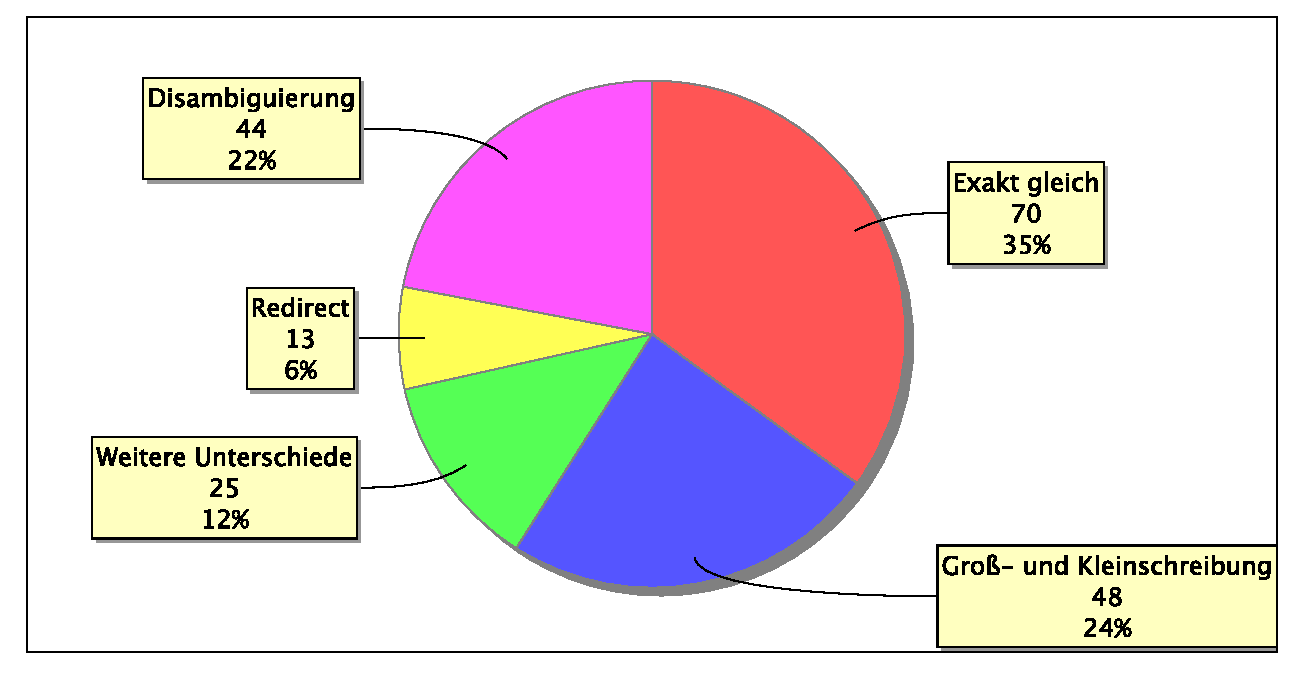
\includegraphics[width=\textwidth]{wortschatz2dbpedia/analyse/mapping1/stichprobe1/wortschatz2dbpedia.analyse.GeneralClassifier.piechart.eps}
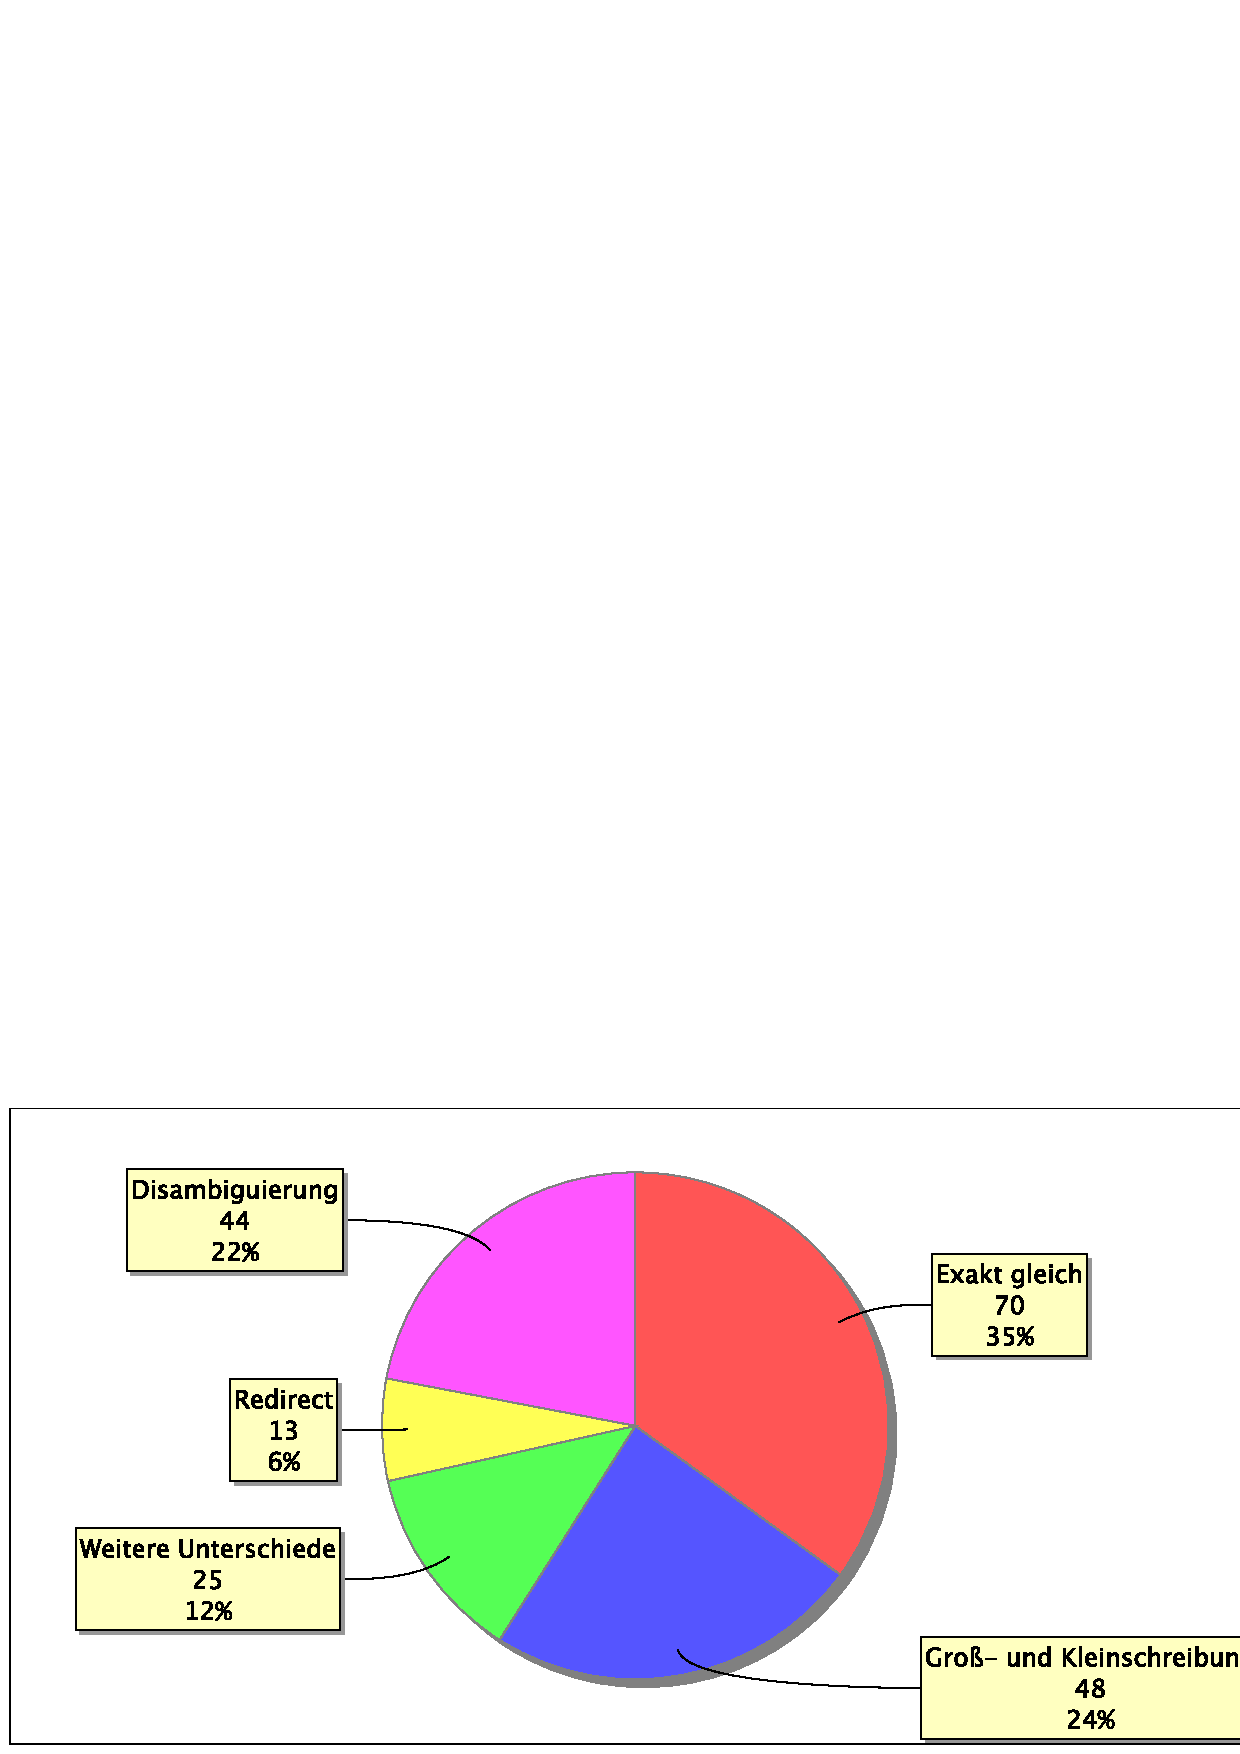
\includegraphics[width=\textwidth]{img/pdf/wortschatz2dbpedia.analyse.GeneralClassifier.piechart.pdf}
\subparagraph*{Genauigkeit}~\\
%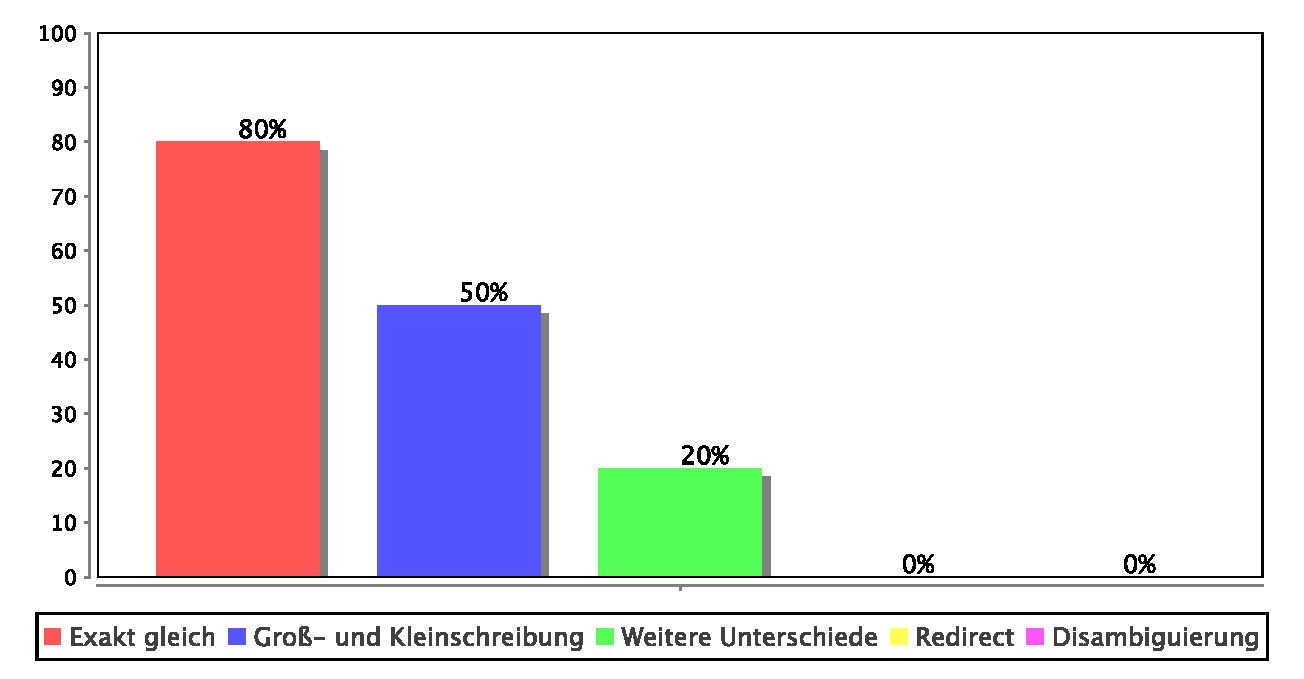
\includegraphics[width=\textwidth]{wortschatz2dbpedia/analyse/mapping1/stichprobe1/wortschatz2dbpedia.analyse.GeneralClassifier.barchart.eps}
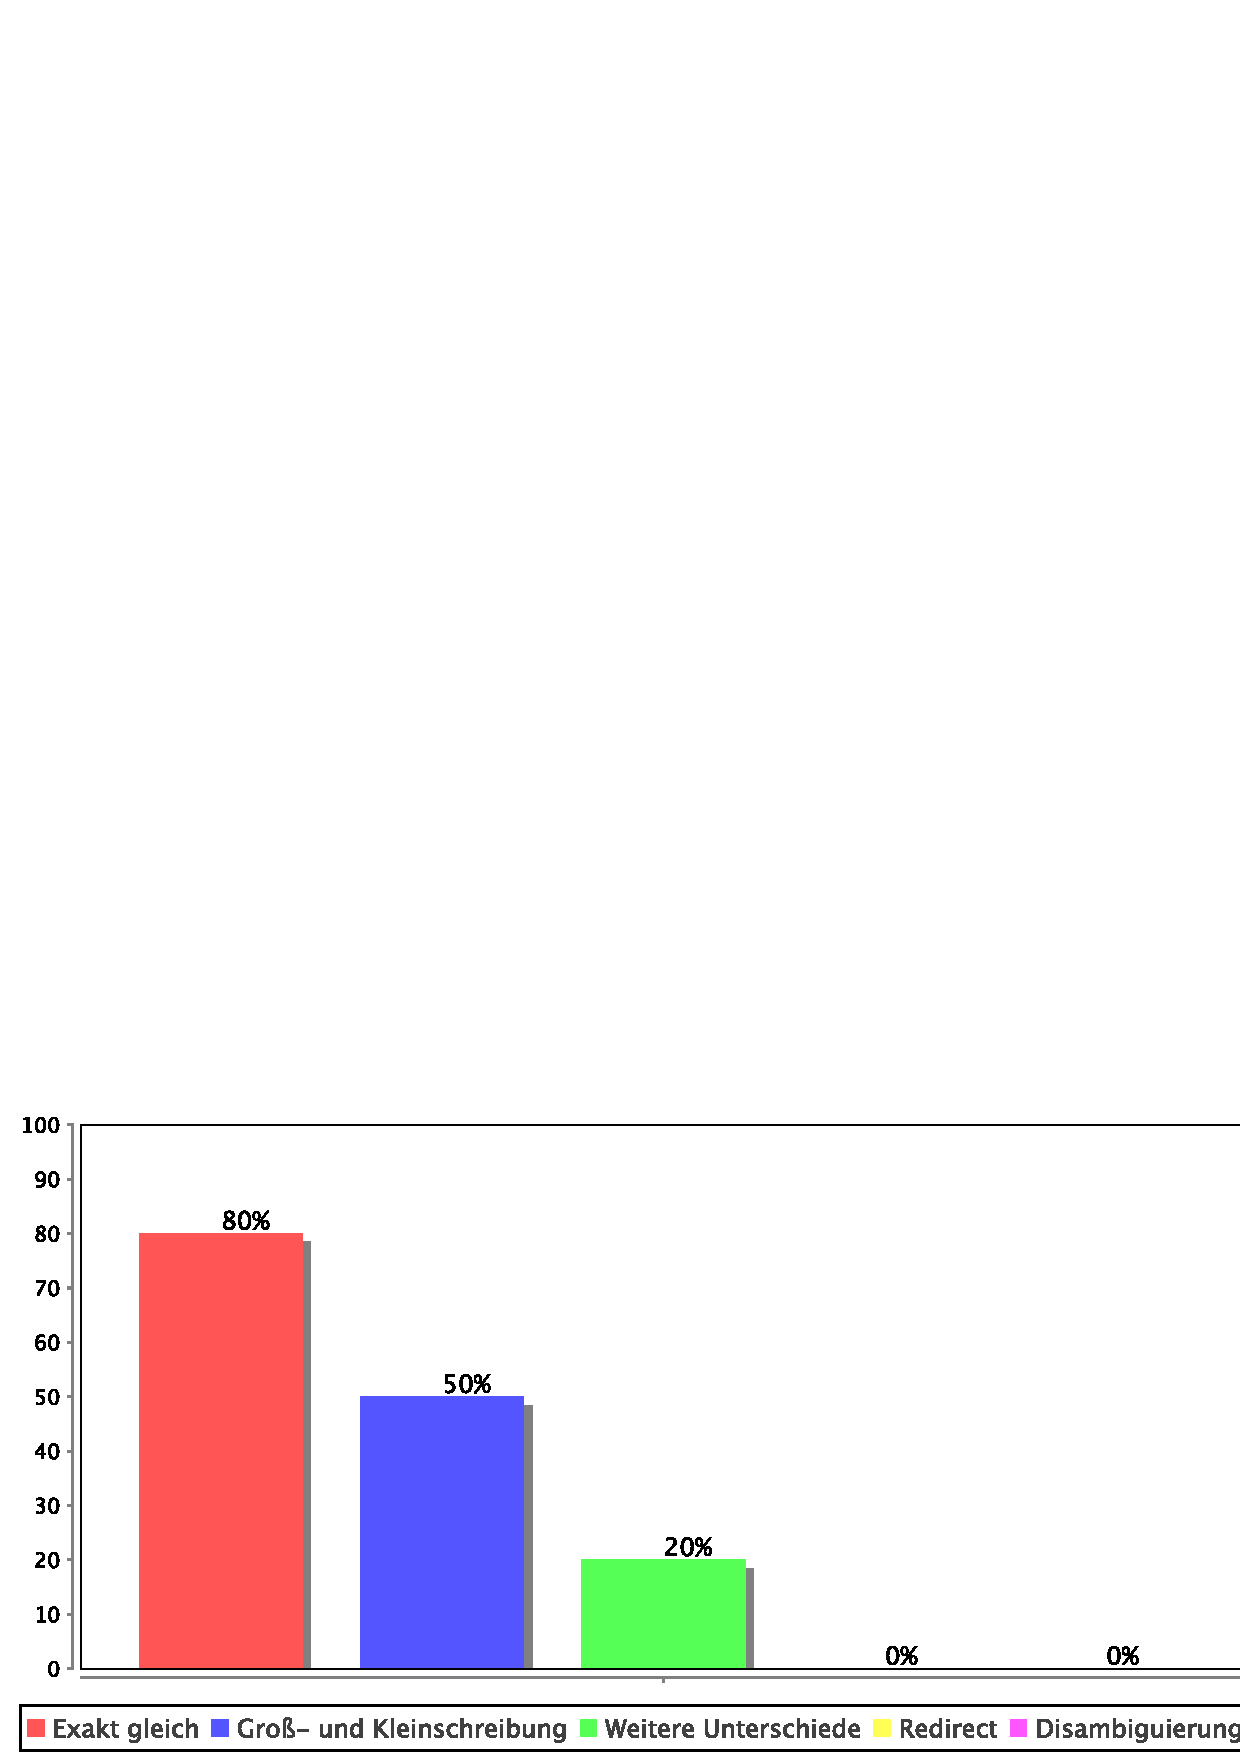
\includegraphics[width=\textwidth]{img/pdf/wortschatz2dbpedia.analyse.GeneralClassifier.barchart.pdf}

Zur Zeit der Analyse wurden Disambiguationsseiten und Redirects in der DBpedia noch nicht einheitlich behandelt.
Grundsätzliche Direktive bei der Extraktion von Artikeln aus der Wikipedia ist es, dass das Label der DBpedia-Ressource zu einem Artikel mit dessen Titel übereinstimmt.
Aus diesem Grund wird, um auch Disambiguierungsseiten (Seiten für mehrdeutige Begriffe, wie \zb{} \emph{Bank}) zu erkennen, der String "`(disambiguation)"' beim Matching ignoriert.
Dies erlaubt, dass auch ein Paar wie (\emph{Time\_(disambiguation)},\emph{Time}) gefunden wird. Zur Zeit der Erstellung des ersten Mappings wurde der String "`(disambiguation)"' jedoch in vielen Fällen 
bei der Extraktion der Wikipedia zur DBpedia entfernt. Die DBpedia-Ressource mit "`(disambiguation)"' im Titel existierte jedoch trotzdem noch, nur dass sie keinen Inhalt hatte.
Nachfragen ergaben jedoch, dass dies später behoben werden sollte, sodass am Matching nichts verändert, beim Betrachten der Stichproben Disambiguierungen jedoch außen vor gelassen werden.
Weiterhin existierten auch zu einigen Redirects DBpedia-Entitäten, die eigentlich in einem anderen Datenset sind. Da auch dies behoben werden sollte, werden auch die Redirects aus der Stichprobenbetrachtung
ausgeklammert.
%Einträge, die auf Disambiguierungsseiten (43 Einträge) oder Redirects (13 Einträge) verwiesen, waren deshalb fehlerhaft.
Von nun an werden nur die restlichen 144 Einträge betrachtet, die geschätzte Genauigkeit dieser Teilmenge beträgt $\valunit{59}{\%}$. Das $\valunit{95}{\%}$-Konfidenzintervall beträgt $[73,97]$,
also $[\valunit{50.6}{\%},\valunit{67.4}{\%}]$.
%\footnote{Linke Grenze abgerundet, Rechte Grenze aufgerundet auf zwei Stellen hinter dem Komma. Dies gilt für alle Konfidenzintervalle in dieser Arbeit.
%Alle anderen Werte sind auf zwei Nachkommastellen mathematisch (geodätisch) gerundet.}.
Im Folgenden wird die Zusammensetzung der Stichprobe und die Genauigkeit der einzelnen Teile genauer aufgeschlüsselt.
\subsection{Unterschiede in der Groß- und Kleinschreibung}

%Da Wikipediaartikeltitel immer mit einem Großbuchstaben anfangen, können folgende Fälle auftreten:
\iffalse
\begin{center}
\begin{tabular}{p{4cm}lll}
Unterschiede& \multicolumn{2}{l}{Beispiel} \\
\hline
keine				&Baird  	&Baird\\
erster Buchstabe\footnotemark	&Mandolin  	&mandolin\\
weitere Buchstaben		&AirPort  	&Airport\\
\hline
alles Andere			&Théodore 	&Theodore\\
\end{tabular}
\end{center}
\footnotetext{Da Wikipediaartikeltitel immer mit einem Großbuchstaben anfangen, handelt es sich in diesem Fall immer um ein kleingeschriebenes Wortschatzwort.}
\newpage
\fi
\subparagraph*{Häufigkeit}~\\
%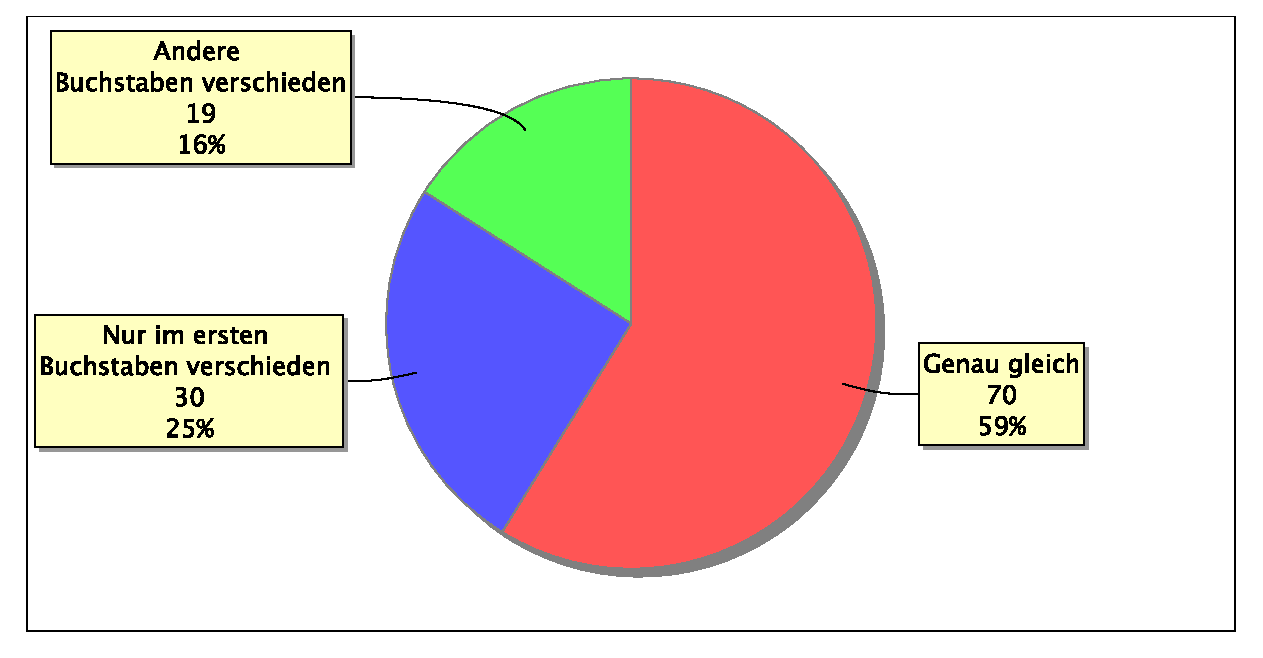
\includegraphics[width=\textwidth]{wortschatz2dbpedia/analyse/mapping1/stichprobe1/wortschatz2dbpedia.analyse.CaseClassifier.piechart.eps}
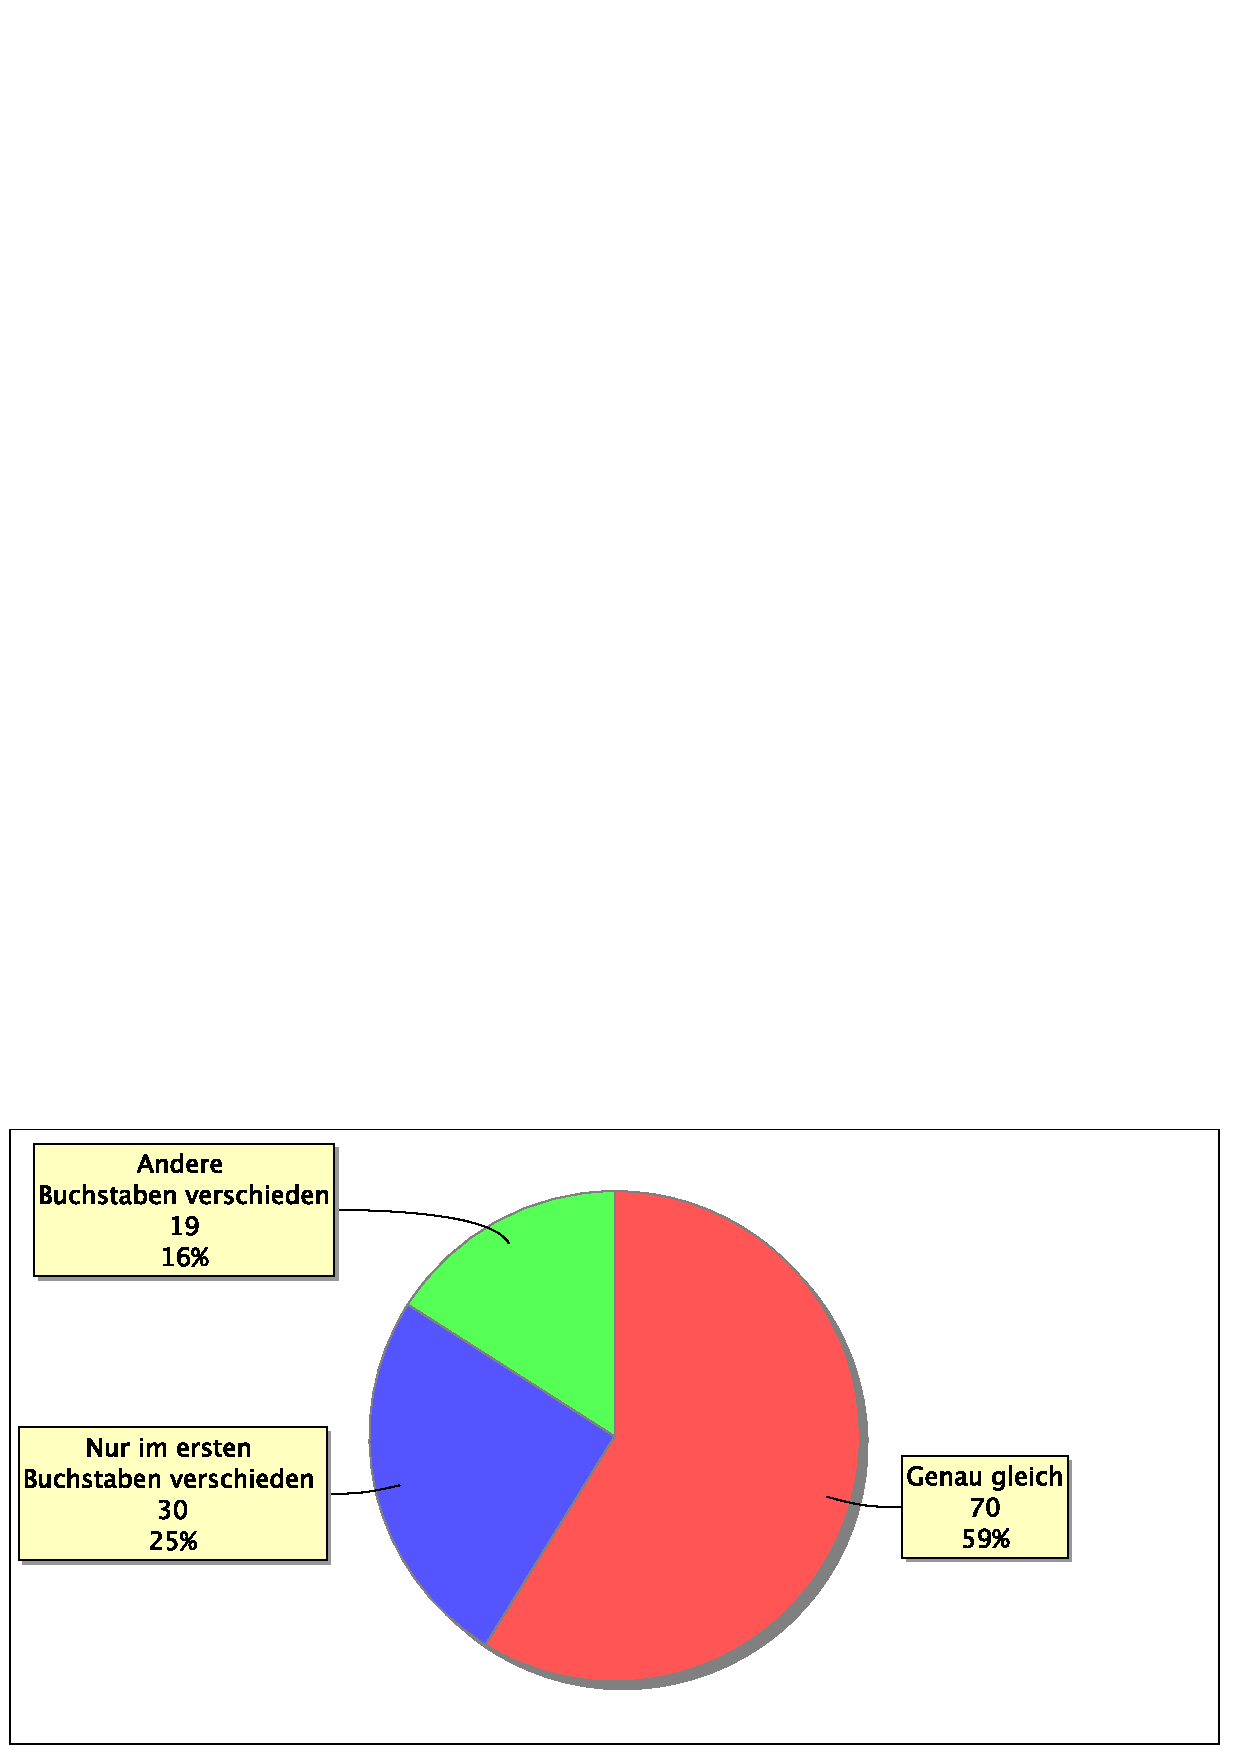
\includegraphics[width=\textwidth]{img/pdf/wortschatz2dbpedia.analyse.CaseClassifier.piechart.pdf}
\subparagraph*{Genauigkeit}~\\
%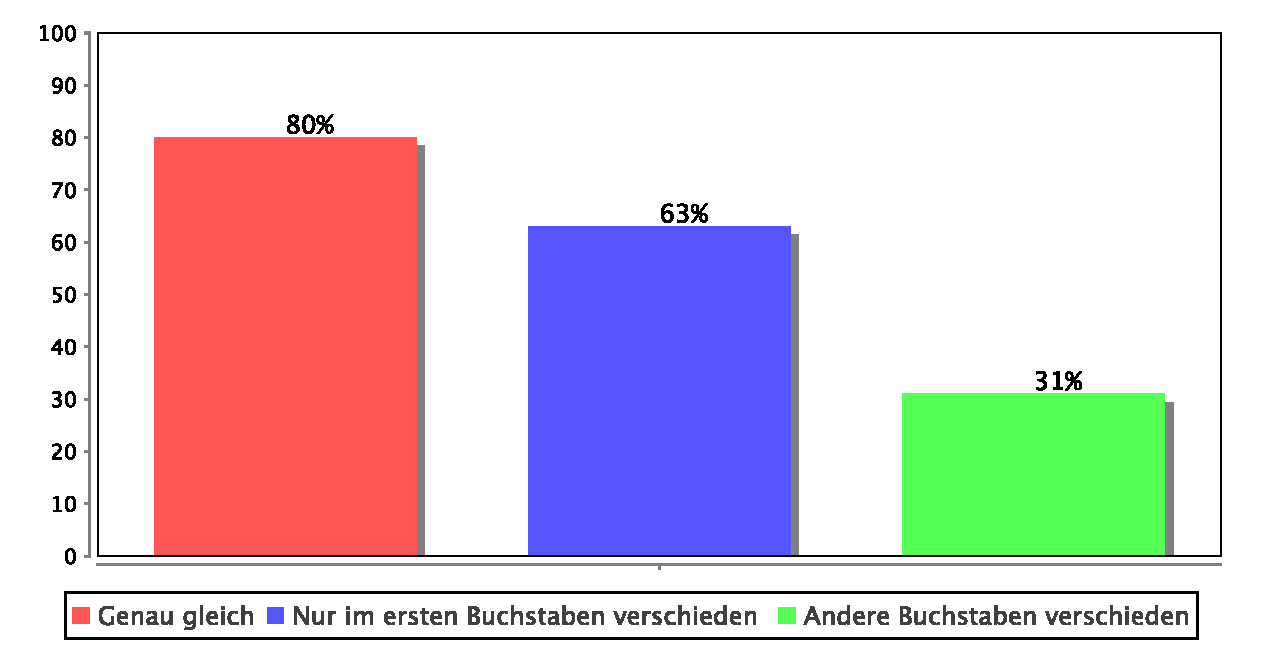
\includegraphics[width=\textwidth]{wortschatz2dbpedia/analyse/mapping1/stichprobe1/wortschatz2dbpedia.analyse.CaseClassifier.barchart.eps}
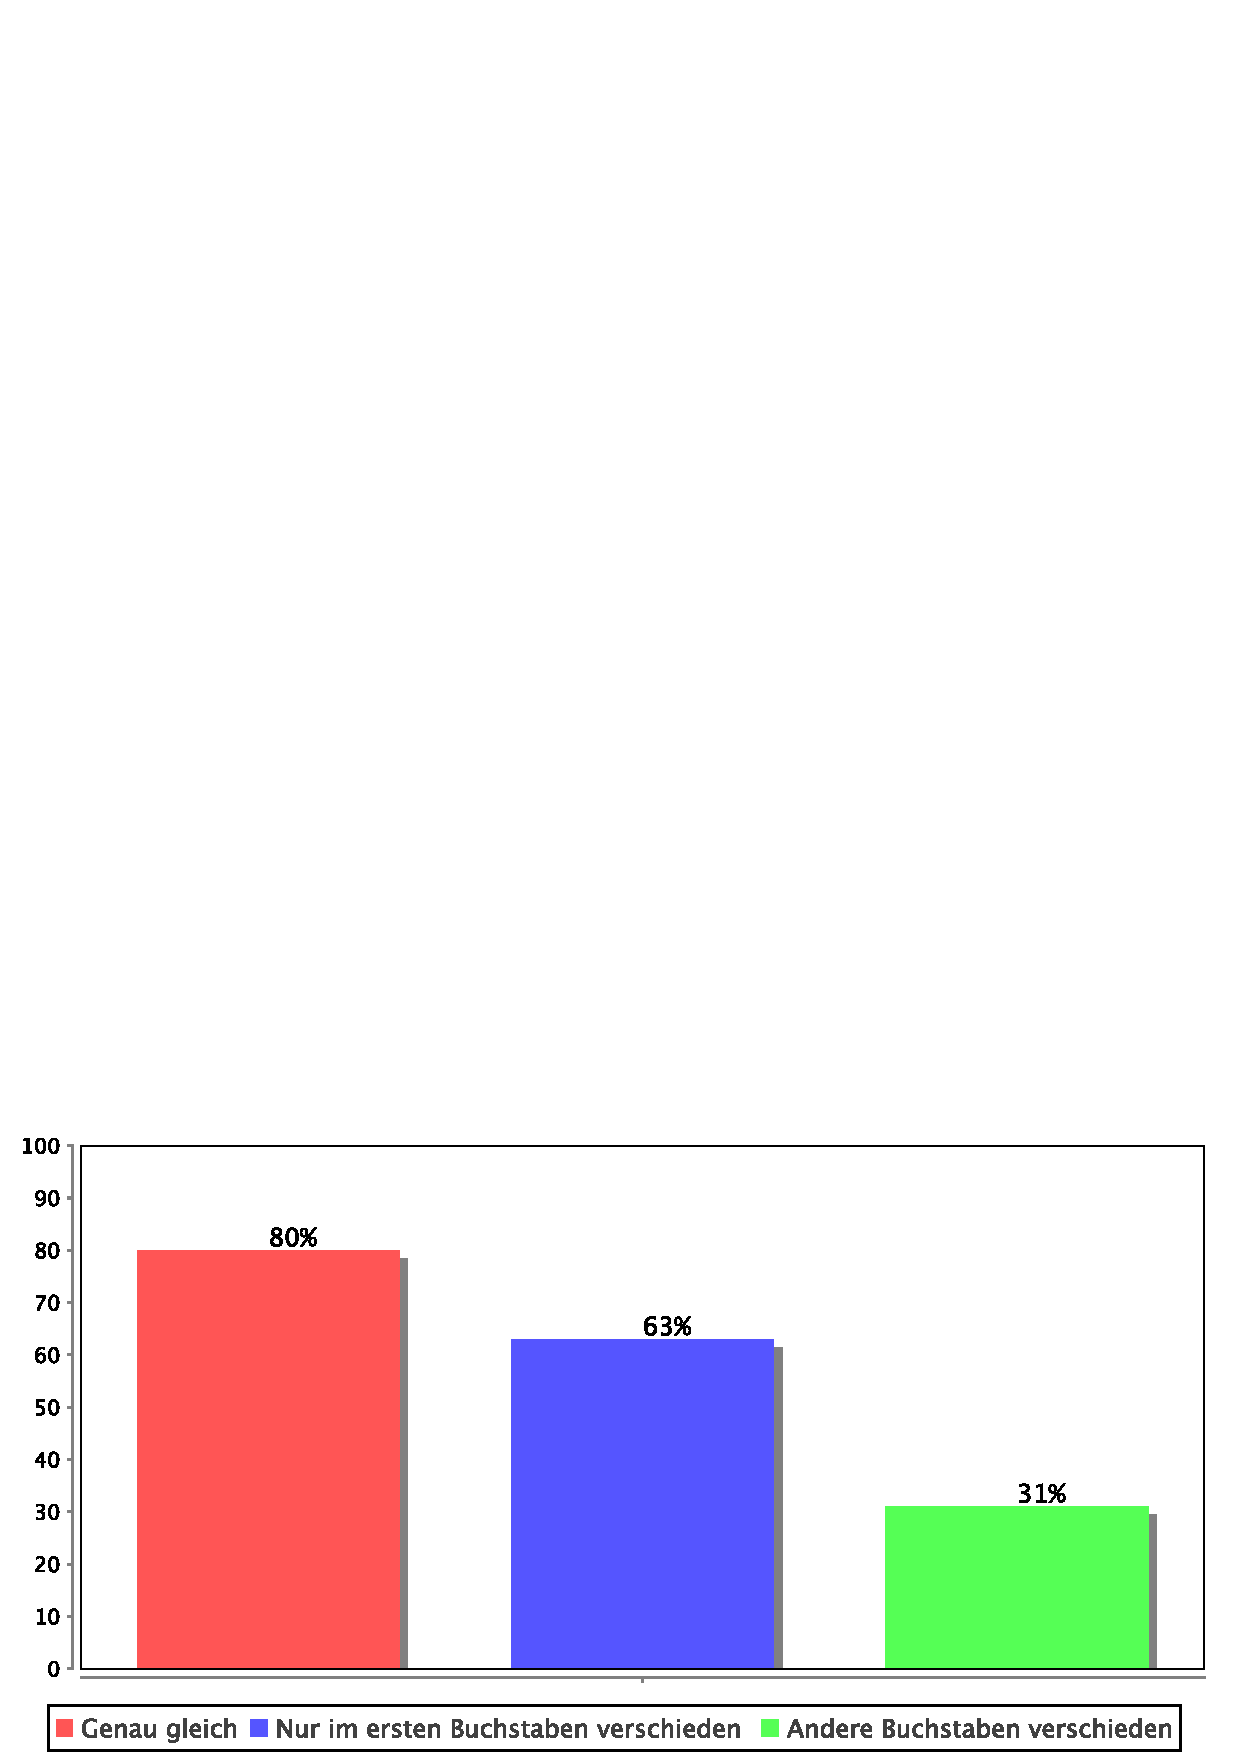
\includegraphics[width=\textwidth]{img/pdf/wortschatz2dbpedia.analyse.CaseClassifier.barchart.pdf}
Obwohl der Artikelname immer groß geschrieben und dessen eigentliche Großschreibung daher unbekannt ist,
gibt es eine deutliche Differenz zwischen der Genauigkeit von \valunit{80}{\%} bei groß geschriebenen und \valunit{63}{\%} bei klein geschriebenen Wörtern des Wortschatzes.
Dies wird damit erklärt, dass Wikipedia eher Artikel über spezielle Begriffe, also vor allem Eigennamen, enthält, die im englischen groß geschrieben werden.
Sucht man also zu einem beliebigen Wort aus dem Wortschatz ein passendes Gegenstück in der DBpedia, dann wird dieses Gegenstück mit einer höheren Wahrscheinlichkeit ein Eigenname und damit 
im normalen Sprachgebrauch groß geschrieben sein.
% Nach dem Erstellen dieser Analyse fiel auf, dass die Betrachtung der Groß- und Kleinschreibung anhand des Artikelnamens wenig aussagekräftig ist, da sowohl der Artikelname als 
% auch der Artikeltitel immer mit einem Großbuchstaben anfangen. Es kann also passieren, dass der DBpedia-Artikelname eigentlich klein geschrieben wird und somit ein klein geschriebenes Wort 
% aus dem Wortschatz fälschlicherweise als nicht exakt passend oder ein groß geschriebenes Wortschatzwort fälschlicherweise als exakt passend deklariert wird.

% In der Anforderungsanalyse in Abschnitt \ref{sec:anforderungen} wird eine Unterteilung in Korrespondenzen hoher und niedriger Präzision festgelegt.
% Beim Betrachten der Daten wird augenscheinlich, dass nur die exakten Übereinstimmungen über eine ausreichend hohe Präzision für den ersten Typen verfügen.
% Der Unterschied in der Genauigkeit zwischen den Wörtern, die im nur Ersten, und denen, die auch in anderen Buchstaben Unterschiede in der Großschreibung aufweisen, ist jedoch auch noch sehr groß.
 Die Präzision der Wörter mit beliebigen Unterschieden in der Großschreibung ist mit \valunit{31}{\%} selbst für eine unsichere Verknüpfungen zu niedrig.
% Lässt man den Nutzer im Wortschatz zwischen mehreren Alternativen wählen, so könnte so ein Link jedoch durchaus nützlich sein. Gegen eine Aufnahme dieser Paare sprechen dennoch folgende Gründe:
\iffalse
\begin{enumerate}
\item würde dadurch die immer noch gute Genauigkeit der anderen Verknüpfungen gemindert
\item würden bei einer Häufigkeit von \valunit{16}{\%} und einer Genauigkeit von \valunit{31}{\%} die hinzukommenden korrekten Paare nur \valunit{4.96}{\%} der Größe des bisherigen Mappings betragen
\item würde dann ein dritter Linktyp ("`ganz unsicher"') nötig werden, dies lohnt sich aufgrund der geringen Anzahl dieser Kategorie jedoch nicht und würde den Prozess nur unnötig verkomplizieren
\end{enumerate}
\fi
% \subparagraph{Schlußfolgerung}
% Um dieses Manko zu beheben, wird die Großschreibung des Begriffs bei DBpedia anhand des Abstracts ermittelt.
% Eine Liste sämtlicher Abstracts ist auf der Seite der DBpedia im Format N3 herunterladbar\footnote{\url{http://wiki.dbpedia.org/Downloads}}.
% Ist das Wort im Abstract überwiegend klein geschrieben, dann wird das Wort als klein geschrieben definiert.
% Anderenfalls (also auch bei Gleichstand und wenn es dort gar nicht vorkommt) wird es als groß geschrieben definiert.
% Vorkommen des Wortes am Satzanfang werden dabei ignoriert.

%Die exakten Matches werden als Links mit hoher Präzision aufgenommen, diejenigen, deren Groß- und Kleinschreibung sich unterscheidet als Links mit niedriger Präzision.
% Einträge mit Unterschieden in der Großschreibung über den ersten Buchstaben hinaus werden nicht aufgenommen.
%Da jedoch keine genaue Grenze für den zweiten Typen festgelegt wurde, fiel die Entscheidung schwer, ob 
%Im Vorhinein wurde keine bestimmte Grenze für die Genauigkeit festgelegt. Ist nur die Großschreibung des ersten Buchstabens verschieden, 
\subsection{Sonderzeichen}
Nach einer kurzen Sichtung der Stichprobe wurden die Wörter, die Sonderzeichen enthalten, in die folgenden Kategorien unterteilt:
\begin{center}
\begin{tabular}{p{4cm}lll}
\toprule
Kategorie& \multicolumn{2}{l}{Beispiel} \\
\midrule
Akzente und Umlaute		&\stichprobentabelleninneres{Théodore}  	&\stichprobentabelleninneres{Theodore}\\
~				&\stichprobentabelleninneres{Mädchen}		&\stichprobentabelleninneres{Madchen}\\
\midrule
Striche				&\stichprobentabelleninneres{Subcontractor}	&\stichprobentabelleninneres{sub-contractor}\\
~				&\stichprobentabelleninneres{MK801}		&\stichprobentabelleninneres{MK-801}\\
\midrule
Punkte				&\stichprobentabelleninneres{D.b.s.}		&\stichprobentabelleninneres{DBs}\\
				&\stichprobentabelleninneres{D.I.R.T.}		&\stichprobentabelleninneres{dirt}\\
				&\stichprobentabelleninneres{K.I.N.G.}		&\stichprobentabelleninneres{king}\\
\midrule
Mehrere davon			&\multicolumn{2}{c}{In der Stichprobe nicht vorhanden}\\
\midrule
Anderes				&\stichprobentabelleninneres{Cat}		&\stichprobentabelleninneres{\`cat}\\
~				&\stichprobentabelleninneres{Waryś}		&\stichprobentabelleninneres{WARY}\\
~				&\stichprobentabelleninneres{Jihâd}		&\stichprobentabelleninneres{`jihad}\\
~				&\stichprobentabelleninneres{Mârşa}		&\stichprobentabelleninneres{Mara}\\
\bottomrule
\end{tabular}
\end{center}

\subparagraph{Häufigkeit}~\\
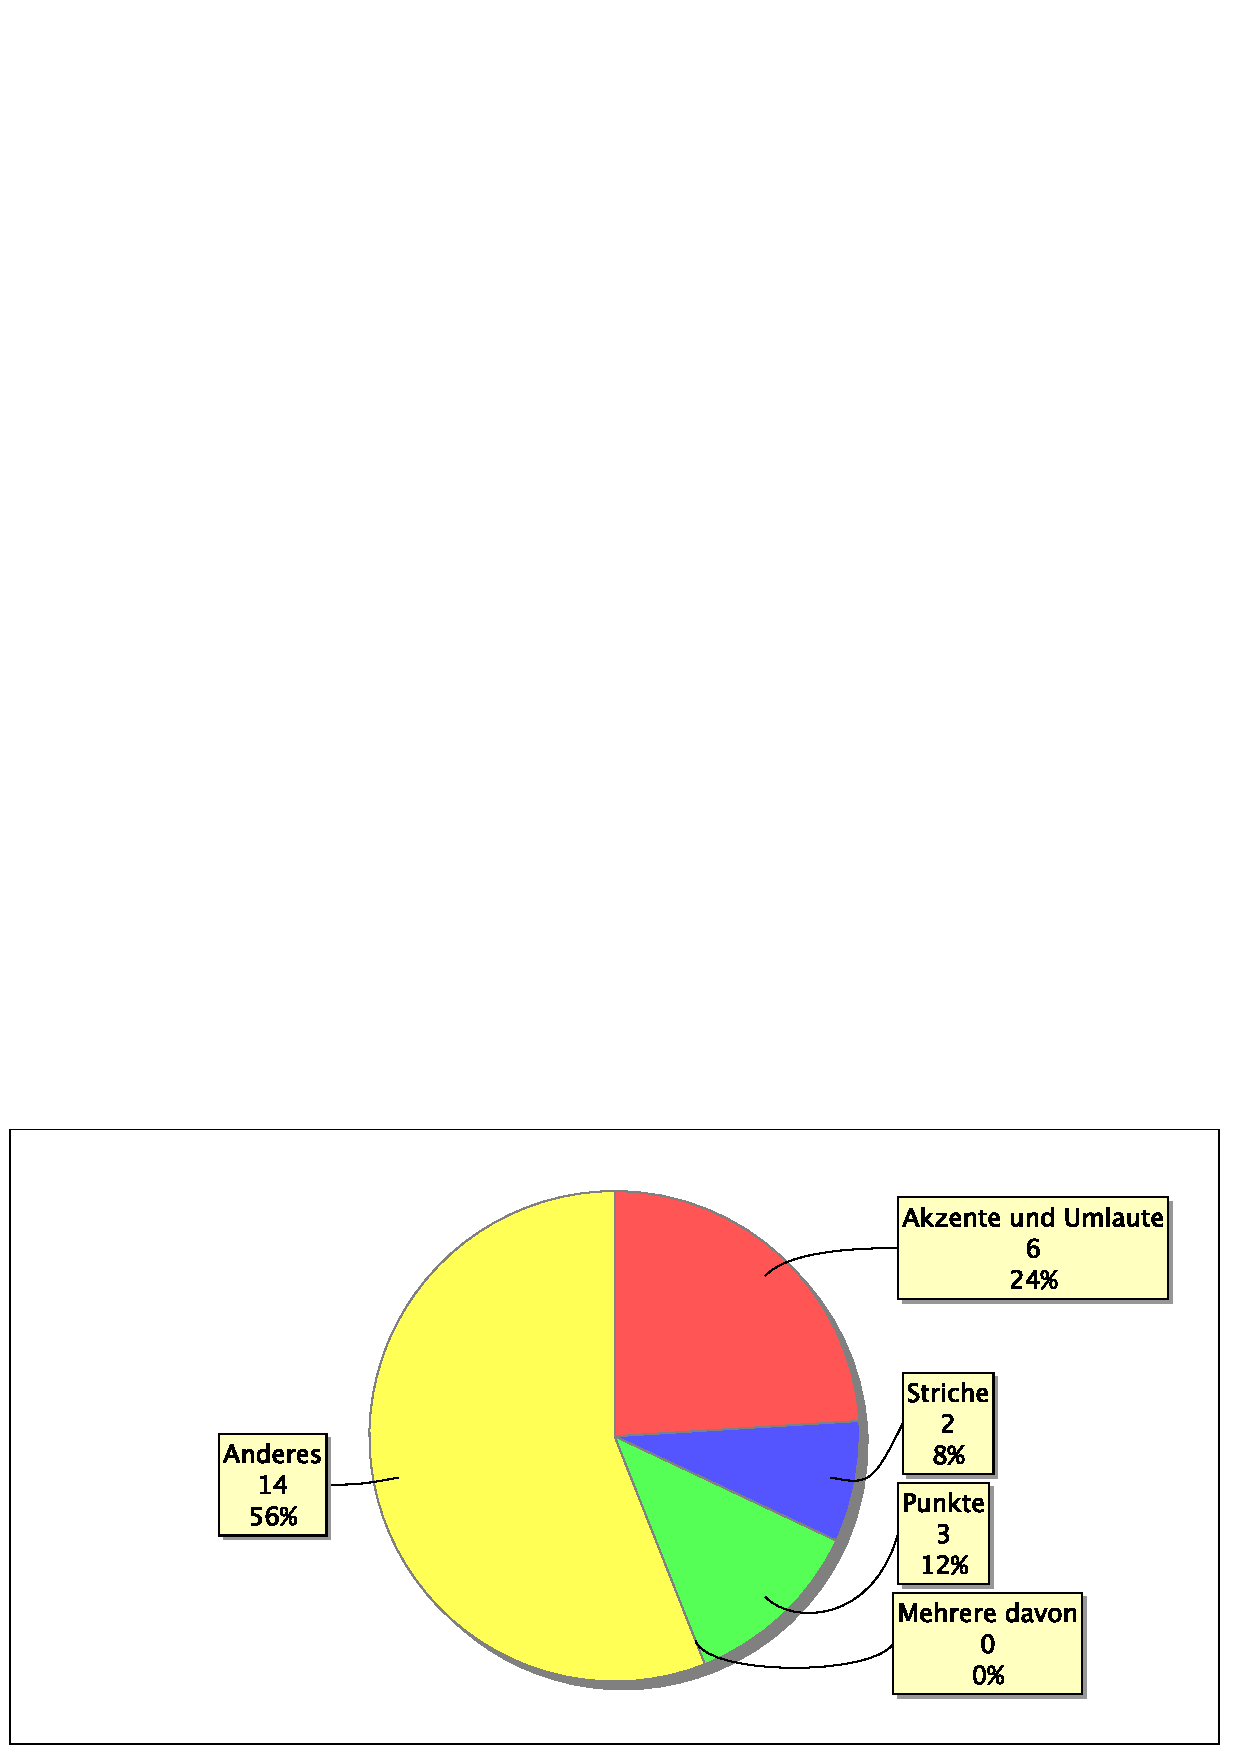
\includegraphics[width=\textwidth]{img/pdf/wortschatz2dbpedia.analyse.SpecialCharactersClassifier.piechart.pdf}
\subparagraph{Genauigkeit}~\\
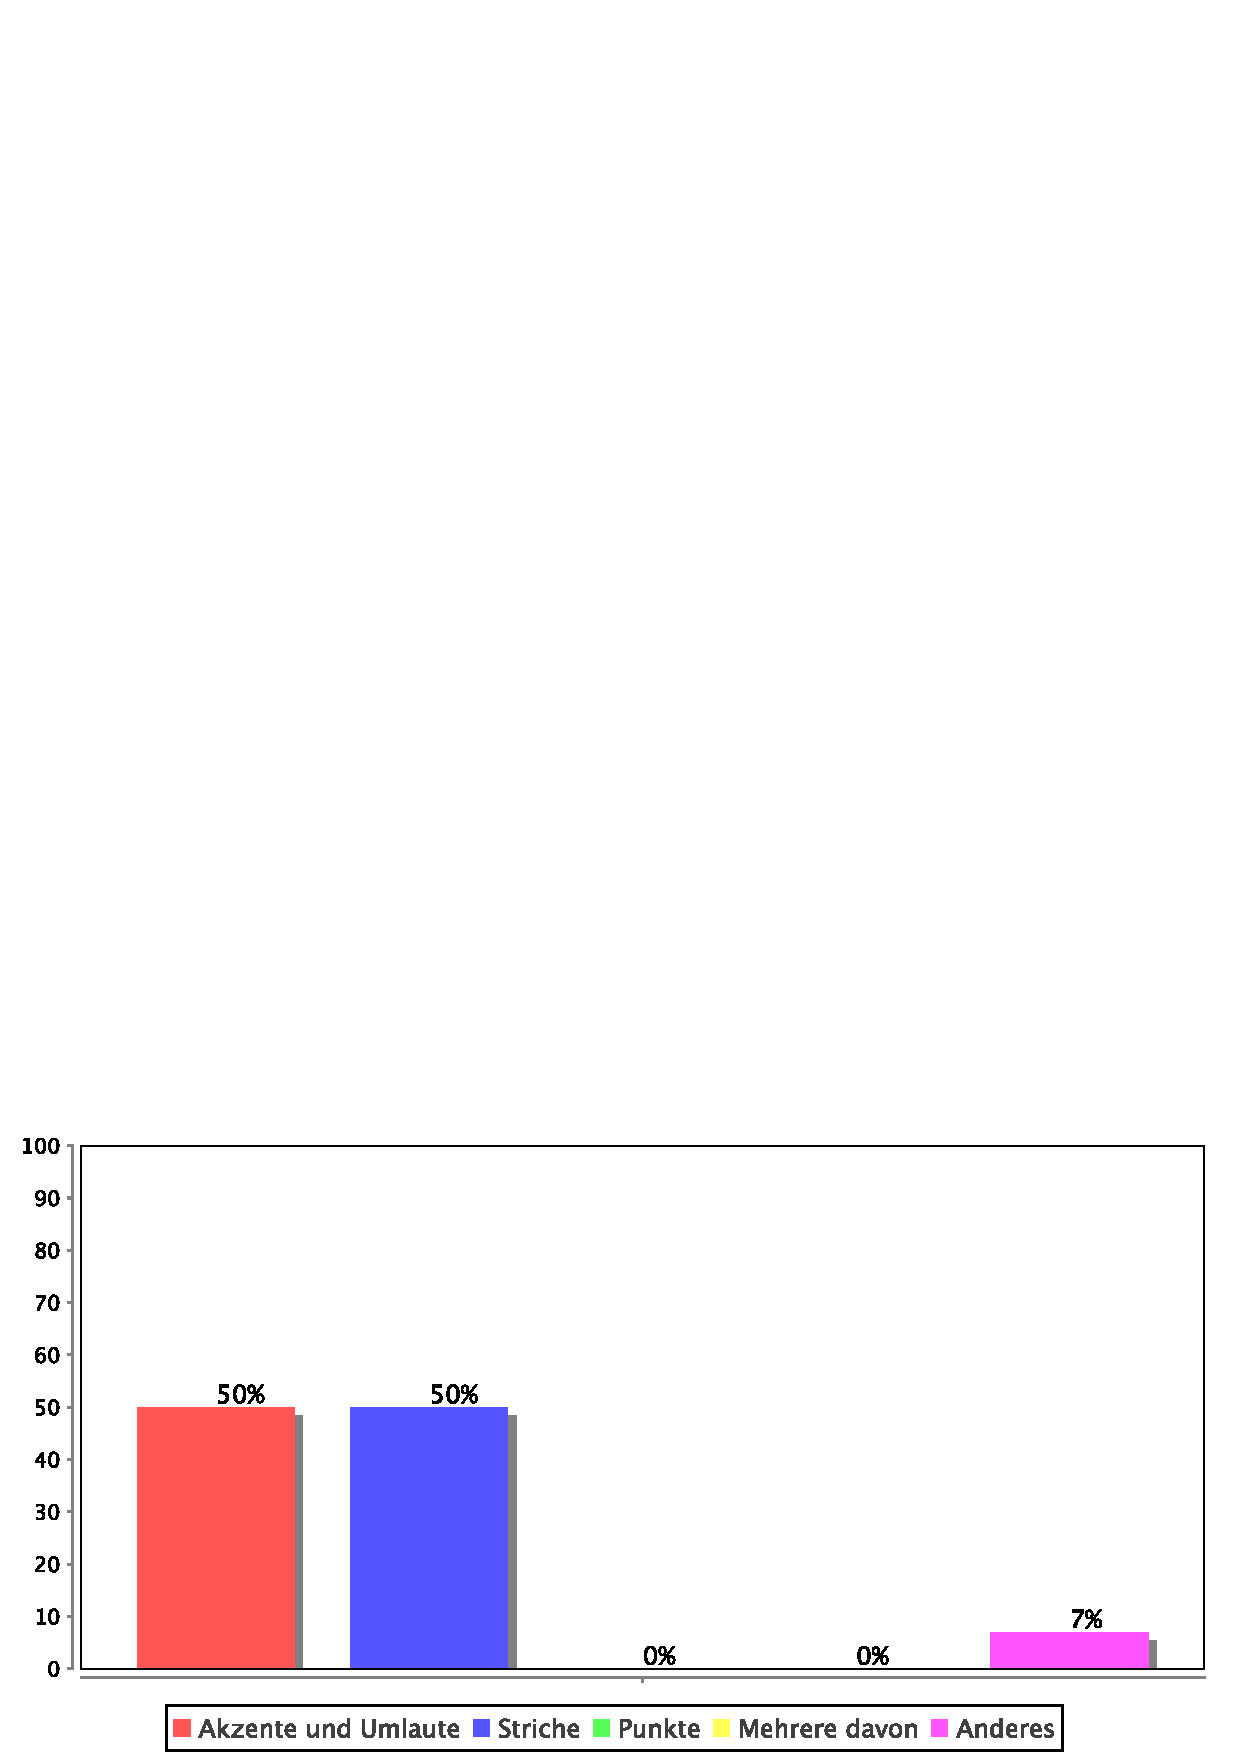
\includegraphics[width=\textwidth]{img/pdf/wortschatz2dbpedia.analyse.SpecialCharactersClassifier.barchart.pdf}
\paragraph{Erweiterte Stichprobe}
Aufgrund der geringen Stichprobenteilgröße ist die Aussagekraft der Einschätzung sehr gering. Außerdem wird bei der Betrachtung der Sonderzeichen in der ersten Stichprobe die Großschreibung ignoriert.
Aus diesem Grund wurde für die drei Kategorien "`\emph{Akzente und Umlaute}"', "`\emph{Striche}"' und "`\emph{Punkte}"' noch je eine weitere zufällige Stichprobe im Umfang von 30 Einträgen untersucht,
bei der nur die Großschreibung des ersten Buchstabens ignoriert wird.
\subparagraph{Akzente und Umlaute}
\begin{table}[h]
\caption{Umwandlungstabelle der Umlaute}
\begin{tabular}{l|l}
\toprule
ÌÍÎÏ		&I\\
ÀÁÂÃÄÅÆ		&A\\
Ç		&C\\
ÈÉÊË		&E\\
Ý		&Y\\
ÙÚÛÜ		&U\\
ÒÓÔÕÖ		&O\\
ìíîï		&i\\
àáâãäåæ		&a\\
ç		&c\\
èéêë		&e\\
ý		&y\\
ùúûü		&u\\
òóôõö		&o\\
\bottomrule
\end{tabular}
\end{table}
%\clearpage%damit die tabelle nicht sonstwo platziert wird (klappt aber auch nicht immer)
%\subparagraph*{Ergebnis}
25 der 30 Einträge sind gültig (keine redirects), Fünf davon korrekt. Die Genauigkeit beträgt also \valunit{20}{\%}, das \valunit{95}{\%}-Konfidenzintervall liegt bei [1,9] $(\valunit{4}{\%},\valunit{36}{\%})$.
\subparagraph{Striche}
23 der 30 Einträge sind gültig, Sieben davon korrekt. Die Genauigkeit beträgt \valunit{30.43}{\%}, das \valunit{95}{\%}-Konfidenzintervall liegt bei [3,11] $(\valunit{13.03}{\%},\valunit{47.83}{\%})$.
\subparagraph{Punkte}
24 der 30 Einträge sind gültig, Einer davon korrekt. Die Genauigkeit beträgt \valunit{4.17}{\%}, das \valunit{95}{\%}-Konfidenzintervall liegt bei [0,3] $(\valunit{0}{\%},\valunit{12.5}{\%})$.
%\subparagraph{Schlußfolgerung}
%Zu klein ist die Genauigkeit der drei Kategorien. Auf eine Aufnahme von Einträgen, die sich in Sonderzeichen unterscheiden wurde also verzichtet.
\subsection{Mapping 1}\label{sec:mapping1}
Die folgenden Parameter wurden aus der Analyse der ersten Stichprobe für ein neues Mapping, Mapping 1, festgelegt:
\begin{itemize}
\item Es werden weiterhin nur DBpedia-Ressourcen und Wortschatzwörter mit einer Länge von mindestens drei Buchstaben in Betracht gezogen.\footnotemark
\footnotetext{Die meisten Wörter der englischen Sprache, zu denen es Artikel in der Wikipedia gibt, haben eine Länge von mindestens drei Buchstaben,
denn die Artikel behandeln selten Verben und Präpositionen, wie \emph{to} und \emph{in}, sondern fast ausschließlich Eigennamen, Objekte und abstrakte Konzepte)}
\item Disambiguierungsmarker werden weiterhin ignoriert (\emph{x\_(disambiguation)} wird also weiterhin wie \emph{x}) behandelt. In das Mapping wird jedoch nicht dieses Paar aufgenommen sondern
die Menge aller Paare $(a,x)$, wobei der Artikel mit dem Namen $a$ eine der Disambiguierungsmöglichkeiten von $x$ ist. Diese Paare werden als unsichere Korrespondenzen aufgenommen.
\item Identische Paare werden als Links mit hoher Präzision definiert. Ist der Artikel ein Redirect, dann wird der Artikelname durch den des Ziels des Redirects ersetzt.
\item Paare, bei denen sich einzig die Großschreibung des ersten Zeichens unterscheidet, werden als unsichere Korrespondenzen aufgenommen.
\item Weitere Paare werden nicht aufgenommen.\footnotemark
\footnotetext{Das mag nach solch einer ausführlichen Analyse etwas enttäuschend anmuten aber weniger ist manchmal mehr.}
\end{itemize}
Die Großschreibung des Artikelnamens wird jedoch nicht mehr als immer groß angenommen, sondern anhand des Abstracts der DBpedia-Entität ermittelt.
Eine Liste sämtlicher Abstracts ist auf der Seite der DBpedia im Format N3 herunterladbar\footnote{\url{http://wiki.dbpedia.org/Downloads}}.
Ist das Wort im Abstract überwiegend klein geschrieben, dann wird das Wort als klein geschrieben definiert.
Anderenfalls (also auch bei Gleichstand und wenn es dort gar nicht vorkommt) wird es als groß geschrieben definiert.
Vorkommen des Wortes am Satzanfang werden dabei ignoriert.

\iffalse
\subsection{Erweiterung zur Groß- und Kleinschreibung}
Nach dem Erstellen dieser Analyse fiel auf, dass die Betrachtung der Groß- und Kleinschreibung anhand des Artikelnamens wenig aussagekräftig ist, da sowohl der Artikelname als 
auch der Artikeltitel immer mit einem Großbuchstaben anfangen. Es kann also passieren, dass der DBpedia-Artikelname eigentlich klein geschrieben wird und somit ein klein geschriebenes Wort 
aus dem Wortschatz fälschlicherweise als nicht exakt passend oder ein groß geschriebenes Wortschatzwort fälschlicherweise als exakt passend deklariert wird.
Interessant ist hier, dass trotzdem ein signifikanter Unterschied hinsichtlich der Genauigkeit besteht (\valunit{80}{\%} bei groß geschriebenen, \valunit{63}{\%} bei klein geschriebenen Wörtern aus dem Wortschatz).
Dies wird damit erklärt, dass Wikipedia eher Artikel über spezielle Begriffe, also vor allem Eigennamen, enthält, die im englischen groß geschrieben werden.
Sucht man also zu einem beliebigen Wort aus dem Wortschatz ein passendes Gegenstück in der DBpedia, dann wird dieses Gegenstück mit einer höheren Wahrscheinlichkeit ein Eigenname und damit 
im normalen Sprachgebrauch groß geschrieben sein.

\begin{rem}
Die Analyse muss streng genommen für jede Sprache wiederholt werden. Aus diesem Grunde wurden hier die einzelnen Schritte auch detailliert und nachvollziehbar aufgeführt.
\end{rem}
\fi